\documentclass[11pt]{article}
\usepackage[margin=1in]{geometry}
\usepackage{graphicx}
\usepackage{amsmath,amssymb}
\usepackage{hyperref}
\usepackage{booktabs}
\usepackage{caption}
\usepackage{parskip}
\usepackage{float}

\title{Slingshot Stepsize Schedules for Conic-Particle Mean-Field Games:\\
Experimental Report}
\author{NDDM Project}
\date{\today}

\begin{document}
\maketitle

\begin{abstract}
We test whether Shugart \& Altschuler's negative-stepsize ``slingshot'' schedules
improve convergence of Chizat's conic-particle algorithms (CP-MDA, $L=1$; CP-MP,
$L=2$) to the Mixed Nash Equilibrium (MNE) of continuous two-player zero-sum games.
Four games are studied: a bilinear game (Shugart's own worked example), Chizat's
documented non-convergence case (a sine/cosine Fourier game on the torus,
``Example 4.1''), and two well-conditioned convex-concave sanity games. The
headline result is a split: slingshot cleanly rescues the bilinear game (duality
gap collapses to machine precision vs.\ vanilla's permanent plateau), but does
\emph{not} rescue Chizat's Fourier game when particles start from a uniform
spread over the whole domain. A warm-start ablation shows this is because the
Fourier game's failure is a \emph{global} basin-of-attraction problem, not the
\emph{local} saddle-cycling problem slingshot's theory addresses. This document
explains the on-disk results layout (Section~\ref{sec:layout}) and walks through
every generated comparison panel (Sections~\ref{sec:bilinear}--\ref{sec:sc_sc}).
Section~\ref{sec:outlook} closes by contrasting this toy-scale study with a
proposed higher-stakes pivot, detailed separately in
\texttt{References/preference\_optimization\_ideas.md}.
\end{abstract}

\tableofcontents

\section{How to read this report}
Every panel below is a $2\times2$ figure produced by \texttt{plot\_results.py}
from the per-iteration CSV logs that \texttt{run\_ablation.py} writes. In each
panel:
\begin{itemize}
  \item \textbf{Top-left}: Nikaido--Isoda duality gap (log scale) --- the primary,
  domain-agnostic certificate of Nash-optimality. Lower is better; this is the
  metric to trust first.
  \item \textbf{Top-right}: summed Wasserstein distance from the current $(\mu,\nu)$
  to the registered \texttt{known\_mne} (log scale), where one is registered.
  Co-primary in general, but \textbf{unsound specifically for the bilinear game}
  (Section~\ref{sec:bilinear-w2-caveat}).
  \item \textbf{Bottom-left}: entropy $H(a)$ of the particle weights --- a secondary
  diagnostic of how concentrated the Fisher--Rao weights have become.
  \item \textbf{Bottom-right}: $\lVert \text{barycenter}\rVert$ (log scale), i.e.\
  $\lVert(\,\mathbb{E}_\mu[x],\ \mathbb{E}_\nu[y]\,)\rVert$ --- secondary, but the
  decisive metric for the bilinear game specifically.
\end{itemize}
\textbf{Color convention throughout: vanilla baseline is purple, slingshot is red.}
All seeds for a given configuration are overlaid in the same color.

\section{Results directory layout}
\label{sec:layout}
The \texttt{results/} tree is partitioned per game, and further split into
sub-regimes where a single game admits more than one meaningful experimental
setup. Every leaf directory contains: one CSV per run
(\texttt{L\{1,2\}\_\{vanilla,slingshot\}\_init-\{uniform,near\_mne\}\_seed\{N\}.csv}),
one \texttt{summary.csv} aggregating final metrics and fitted log-linear rates
across all runs in that directory, and a \texttt{plots/} subfolder holding the
PNG dashboards discussed in this report. A single \texttt{summary\_all.csv} at
the \texttt{results/} root concatenates every summary row across every game.

\subsection{\texttt{results/bilinear/}}
Shugart's own worked example, $f(x,y) = xy$ on a bounded euclidean domain.
\begin{description}
  \item[\texttt{pitfall\_default\_stepsize/}] The run at the \emph{default}
  stepsize calibration. Kept deliberately, with an explanatory
  \texttt{README.md} in the same folder, as a documented negative result:
  bilinear's spectrum is degenerate ($m=M=1$), so both the vanilla stepsize
  ($h=1/\sqrt{M}=1$) and the Chebyshev/slingshot schedule (which collapses to
  the same constant magnitude when $m=M$) pick step size $1.0$ --- far above
  the position-step's adaptive clip cap. Both modes saturate the clip and
  freeze at the domain boundary within a handful of steps, making vanilla and
  slingshot look identical for the wrong reason.
  \item[\texttt{calibrated/}] The same comparison re-run with a deliberately
  small step ($h=0.01$, via \texttt{--eta 0.01} for vanilla and
  \texttt{--m 10000 --M 10000} for slingshot) to stay below clip saturation.
  This is the run that actually isolates slingshot's effect, and produces the
  cleanest positive result in this study.
\end{description}

\subsection{\texttt{results/chizat\_example\_4\_1/}}
Chizat's documented non-convergence case: a sine/cosine Fourier-spectrum
payoff on the torus $[0,2\pi)\times[0,2\pi)$.
\begin{description}
  \item[\texttt{global/}] Particles initialized uniformly at random over the
  whole torus --- Chizat's actual experimental setup. This is the regime in
  which Chizat reports CP-MDA fails to converge.
  \item[\texttt{local/}] Particles warm-started with small Gaussian noise
  around the atoms of the known MNE (\texttt{init\_state\_near\_mne}, noise
  $\sigma=0.01$). This regime isolates whether the failure is \emph{local}
  cycling near the saddle (which slingshot's theory is proven to fix) or
  something else entirely.
\end{description}

\subsection{\texttt{results/convex\_concave/}}
A smooth, strongly-monotone convex-concave sanity game
($f(x,y) \propto \tanh$-type one-sided gradients) on a euclidean domain. No
sub-split: standard vanilla-init runs across both $L=1$ and $L=2$.

\subsection{\texttt{results/sc\_sc/}}
A second, better-conditioned sanity game (``sin--cos'' on a euclidean domain),
included to check that nothing about the implementation itself prevents fast,
clean convergence when the underlying game is easy. No sub-split.

\clearpage
\section{Bilinear game}
\label{sec:bilinear}

\subsection{Pitfall: default stepsize calibration}
\begin{figure}[H]
  \centering
  
\includegraphics[width=0.92\textwidth]{bilinear/pitfall_default_stepsize/plots/L1_init-uniform.png}
  \caption{Bilinear, $L=1$, default stepsize. Vanilla and slingshot are
  visually indistinguishable: both saturate the position-step's adaptive clip
  within a few iterations and freeze at the domain boundary, so the duality
  gap plateaus near $190$--$200$ and entropy collapses almost immediately for
  \emph{both} modes. This is a calibration artifact of bilinear's degenerate
  spectrum ($m=M=1$), not a finding about the sign schedule --- see
  \texttt{results/bilinear/pitfall\_default\_stepsize/README.md}.}
\end{figure}

\subsection{Calibrated comparison}
\begin{figure}[H]
  \centering
  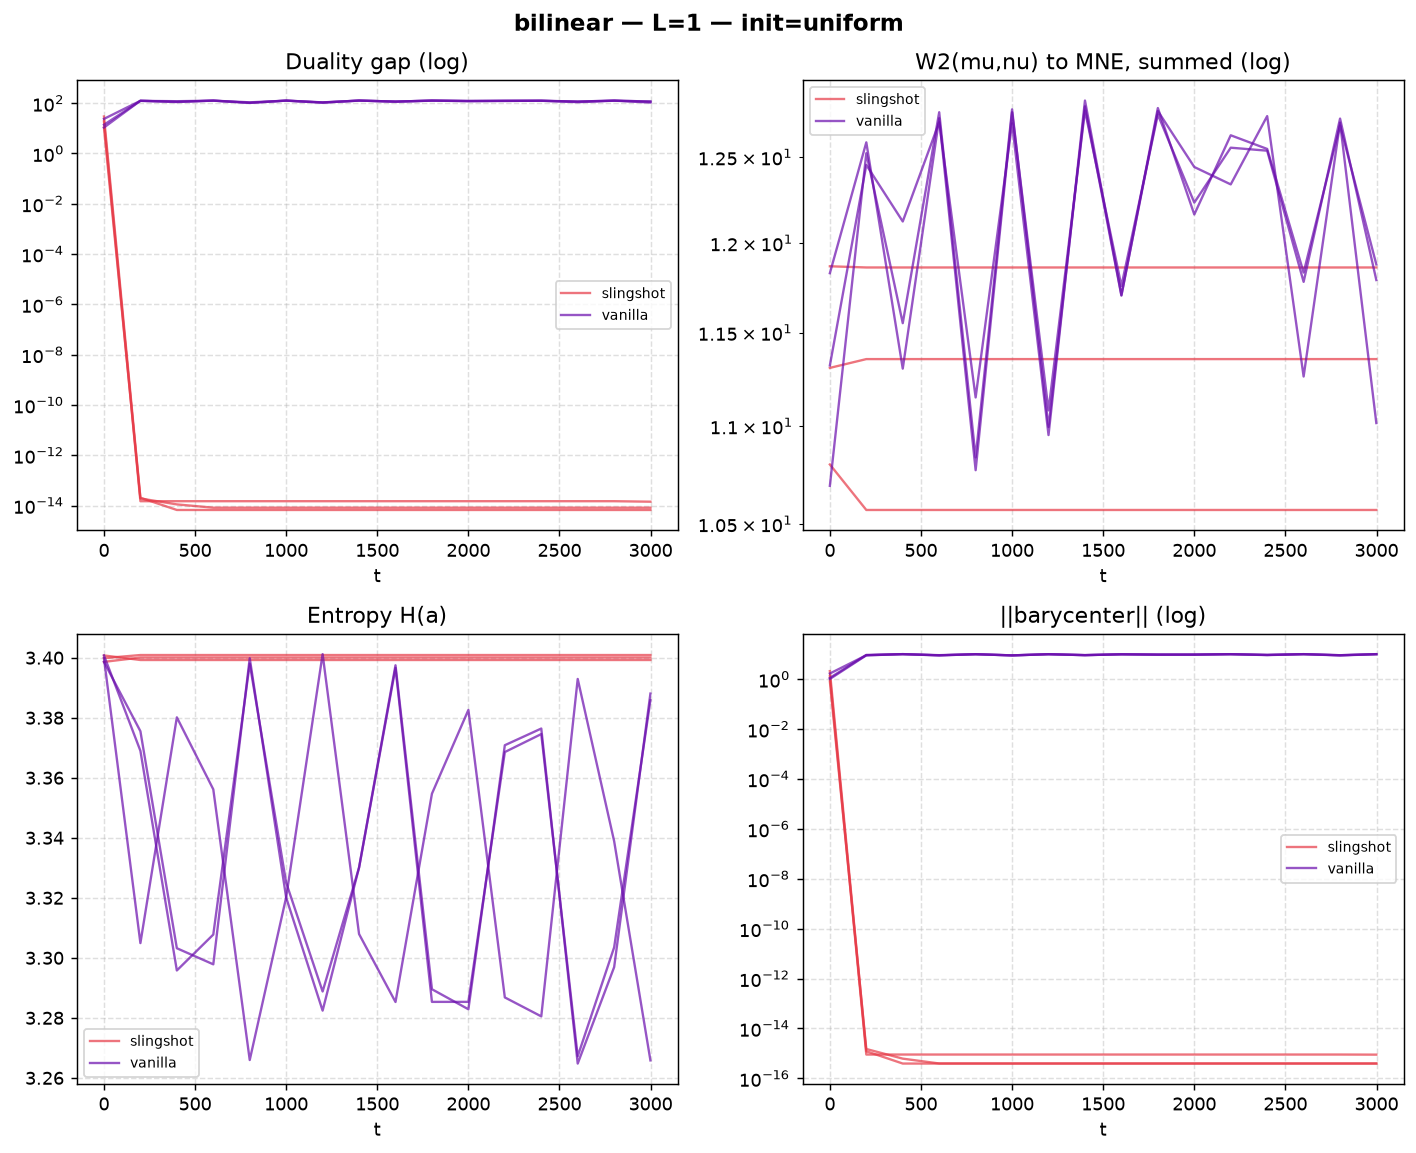
\includegraphics[width=0.92\textwidth]{bilinear/calibrated/plots/L1_init-uniform.png}
  \caption{Bilinear, $L=1$, calibrated stepsize ($h=0.01$, below clip
  saturation). Slingshot's duality gap (red) collapses to machine precision
  ($\sim 10^{-14}$) and stays there; vanilla (purple) stays stuck at
  $\sim 106$--$117$ across all seeds. The barycenter-norm panel tells the same
  story directly: slingshot's barycenter goes to $\sim 10^{-16}$ while
  vanilla's barycenter sits far from zero. This is the cleanest reproduction
  of Shugart's headline claim in this codebase.}
\end{figure}

\subsection{Caveat: the Wasserstein-to-MNE panel is not meaningful here}
\label{sec:bilinear-w2-caveat}
In both bilinear panels above, the top-right (W2-to-MNE) curve stays roughly
flat for \emph{both} modes, which at first looks like a contradiction of the
duality-gap result. It is not a bug. Under product measures, the bilinear
payoff is separable:
\[
  F(\mu,\nu) \;=\; \mathbb{E}_{x\sim\mu}[x]\cdot\mathbb{E}_{y\sim\nu}[y],
\]
so the duality gap depends \emph{only} on the two barycenters, never on the
shape or support of $\mu,\nu$ individually. The true MNE set is therefore the
entire family of zero-mean $(\mu,\nu)$ pairs, not just the single point-mass-at-zero
representative registered as \texttt{known\_mne}. Slingshot's particles spread
out across the domain (individual positions ranging over roughly $[-10, 9.6]$
in the runs here) while their \emph{barycenter} converges exactly to zero ---
so $W_2$ to the canonical representative stays large even though the game is
solved. \textbf{Conclusion: trust the duality gap (and the barycenter panel)
as primary for bilinear; the $W_2$ panel only measures convergence to one
arbitrary representative of the true MNE set, not solution quality.}

\clearpage
\section{Chizat's Fourier game (Example 4.1)}
\label{sec:fourier}

\subsection{Global initialization (Chizat's actual setup)}
\begin{figure}[H]
  \centering
  
\includegraphics[width=0.92\textwidth]{chizat_example_4_1/global/plots/L1_init-uniform.png}
  \caption{Fourier game, $L=1$ (CP-MDA), uniform random initialization over
  the whole torus. Vanilla and slingshot overlap almost exactly: the duality
  gap oscillates in a persistent band with no decay trend, and the entropy
  dips but never collapses --- both modes are cycling/plateauing, not
  converging. This reproduces Chizat's documented non-convergence claim, and
  slingshot provides no visible rescue.}
\end{figure}
\begin{figure}[H]
  \centering
  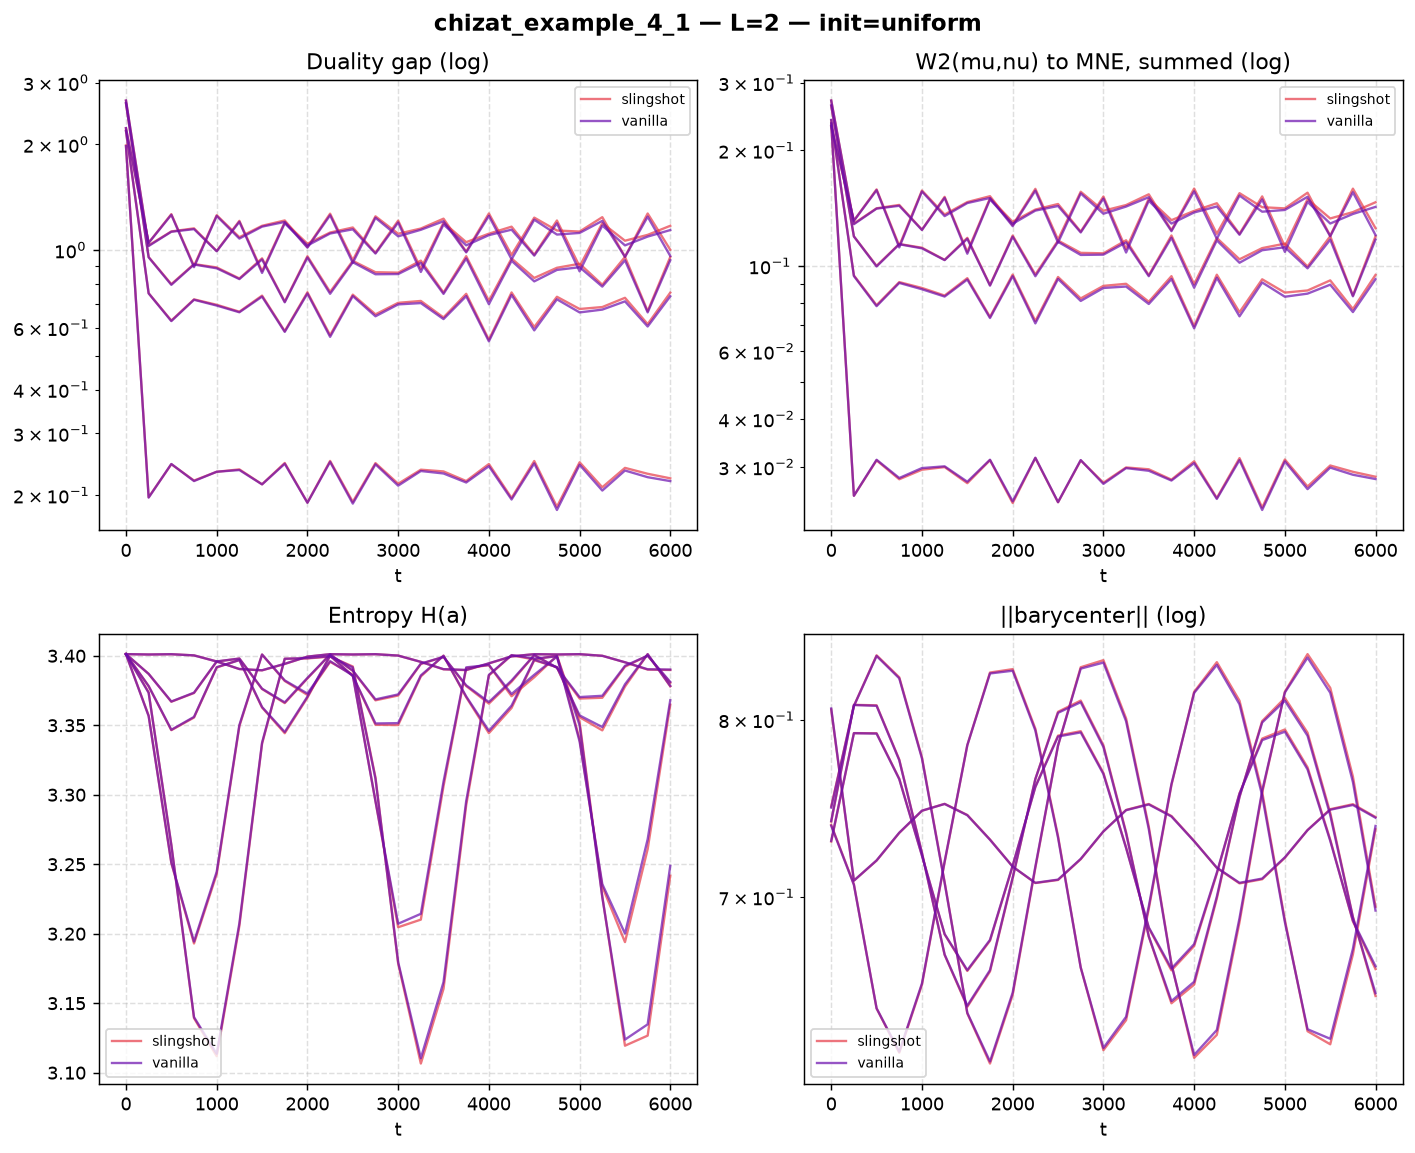
\includegraphics[width=0.92\textwidth]{chizat_example_4_1/global/plots/L2_init-uniform.png}
  \caption{Same setup with $L=2$ (CP-MP / extragradient). The extragradient
  correction does not change the qualitative picture either: both modes still
  plateau without separation.}
\end{figure}

\subsection{Local initialization (warm-started near the known MNE)}
\begin{figure}[H]
  \centering
  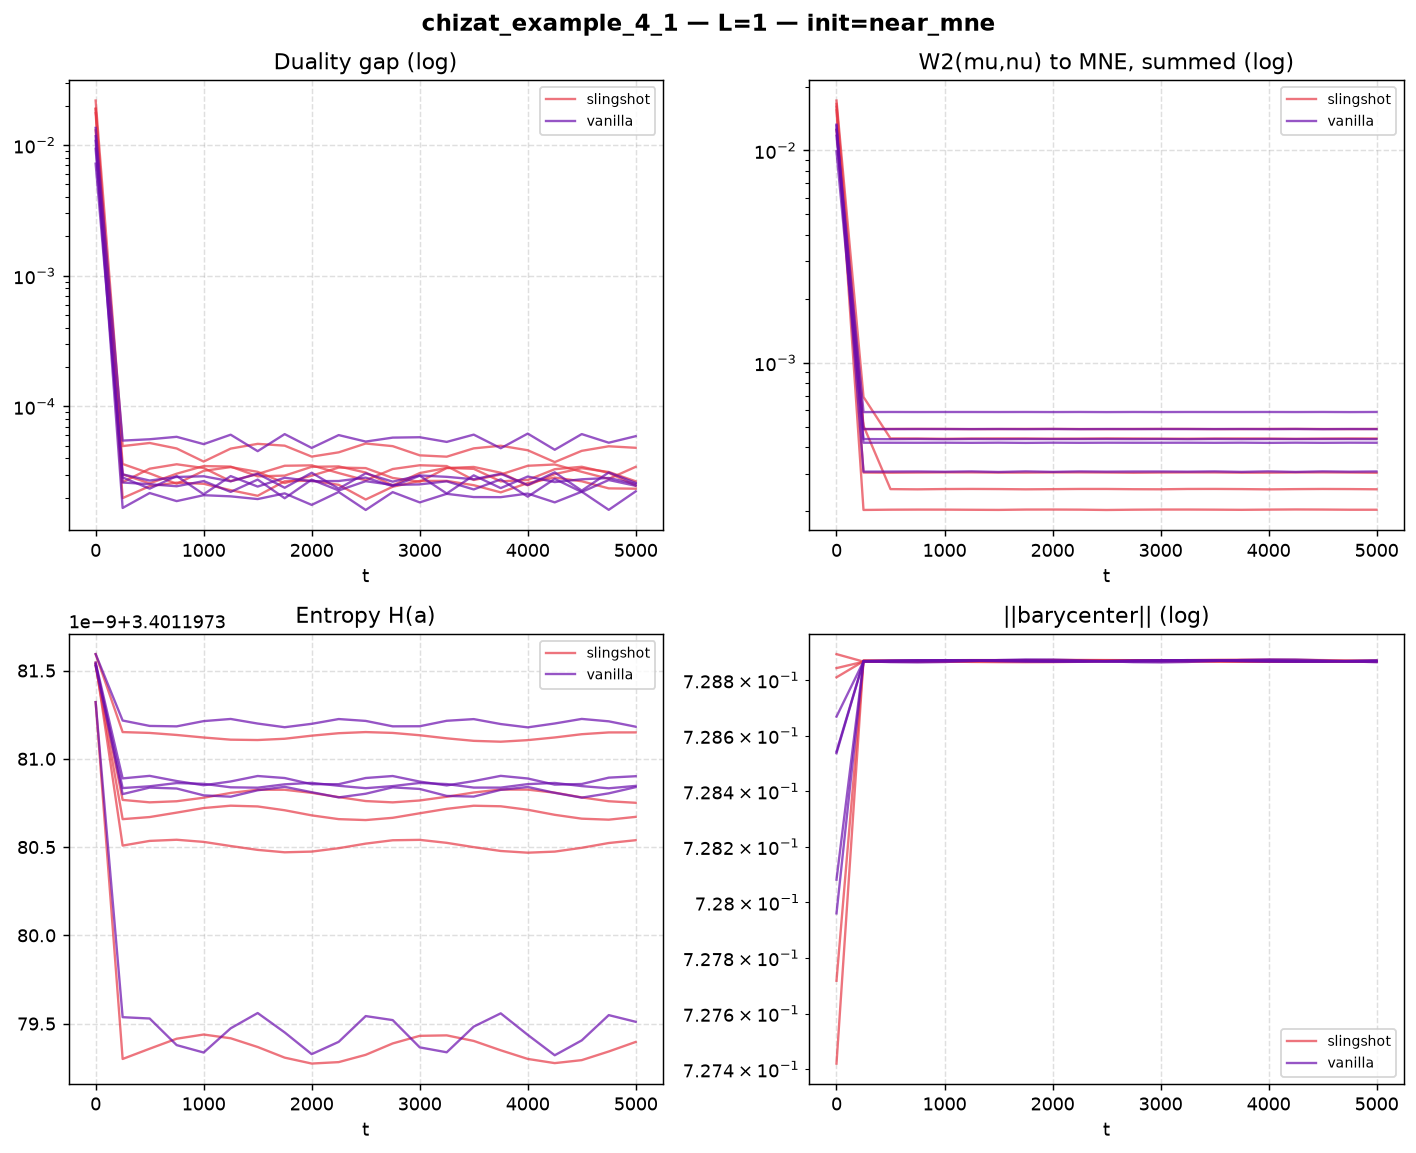
\includegraphics[width=0.92\textwidth]{chizat_example_4_1/local/plots/L1_init-near_mne.png}
  \caption{Fourier game, $L=1$, particles warm-started with small noise
  ($\sigma=0.01$) around the true MNE support. Both modes collapse almost
  immediately to a tiny residual duality gap ($\sim 2.5\times10^{-5}$,
  confirmed not a grid-discretization artifact by comparing
  \texttt{grid\_size}$=400$ vs.\ $2000$) and hold there for the remainder of
  the run. Entropy stays pinned essentially exactly at $\ln(30) \approx 3.4012$
  throughout (only ninth-decimal-place drift), meaning the Fisher--Rao weights
  never needed to move away from the warm-started uniform $1/n$
  initialization --- all the necessary information was already encoded in
  particle \emph{positions}.}
\end{figure}

\subsection{Reading: a global basin-of-attraction failure, not local cycling}
The contrast between the two panels above is the central finding of this
study regarding the Fourier game. Shugart \& Altschuler's slingshot guarantee
is a statement about \emph{local} stability near a saddle: alternating the
sign of the stepsize prevents the kind of small-scale cycling that traps
vanilla gradient descent-ascent near an equilibrium. The local-init panel
shows that once particles are already \emph{near} the right support, neither
mode has any local cycling problem to fix --- they both converge fine,
trivially. The global-init panel shows the real failure mode: starting from a
uniform spread over the whole torus, the Fisher--Rao weight dynamics never
manages to concentrate mass onto the correct support in the first place. That
is a basin-of-attraction / exploration problem, and slingshot's mechanism (a
local position-step sign flip) has no obvious lever on it. This explains why
slingshot does not rescue Chizat's documented failure case: the failure
documented there is not the failure mode slingshot's theory was built to fix.

\clearpage
\section{Convex-concave sanity game}
\label{sec:convex_concave}
\begin{figure}[H]
  \centering
  
\includegraphics[width=0.92\textwidth]{convex_concave/plots/L1_init-uniform.png}
  \caption{Convex-concave game, $L=1$. Both modes converge, with broadly
  similar trajectories.}
\end{figure}
\begin{figure}[H]
  \centering
  
\includegraphics[width=0.92\textwidth]{convex_concave/plots/L2_init-uniform.png}
  \caption{Convex-concave game, $L=2$. Clean, monotone convergence for both
  modes. This is an easy, well-conditioned game by design: it is not the
  regime where vanilla GDA is expected to fail, so the absence of a large
  slingshot advantage here is consistent with theory, not a contradiction of
  the bilinear result.}
\end{figure}

\clearpage
\section{Sin-cos sanity game}
\label{sec:sc_sc}
\begin{figure}[H]
  \centering
  
\includegraphics[width=0.92\textwidth]{sc_sc/plots/L1_init-uniform.png}
  \caption{Sin-cos game, $L=1$. Both modes converge very fast. The duality-gap
  panel's visible $x$-range truncates around $t\approx100$--$150$: once the
  gap drops below the plotting floor, \texttt{plot\_results.py}'s
  \texttt{\_semilogy\_safe} helper masks non-positive/near-zero values before
  taking the log, so the curve simply stops being drawn rather than diving to
  $-\infty$. This is a plotting-floor artifact, not a sign that the run
  stopped early --- it reflects genuinely fast convergence on the
  best-conditioned game in the suite.}
\end{figure}
\begin{figure}[H]
  \centering
  
\includegraphics[width=0.92\textwidth]{sc_sc/plots/L2_init-uniform.png}
  \caption{Sin-cos game, $L=2$. Same fast-convergence picture as $L=1$.}
\end{figure}

\clearpage
\section{Summary of findings}
\begin{description}
  \item[Bilinear] Clean positive result for slingshot once calibrated below
  clip saturation: duality gap to machine precision vs.\ vanilla's permanent
  plateau (Section~\ref{sec:bilinear}).
  \item[Fourier (Chizat 4.1), global init] No rescue: vanilla and slingshot
  are indistinguishable, both plateauing/cycling, reproducing Chizat's
  documented non-convergence claim (Section~\ref{sec:fourier}).
  \item[Fourier (Chizat 4.1), local init] Both modes converge trivially when
  warm-started near the true MNE, showing the global-init failure is a
  basin-of-attraction problem outside the scope of slingshot's local-stability
  guarantee (Section~\ref{sec:fourier}).
  \item[Convex-concave, sin-cos] Both sanity games converge cleanly under both
  modes, as expected for well-conditioned games that are not slingshot's
  target failure case (Sections~\ref{sec:convex_concave}--\ref{sec:sc_sc}).
\end{description}
Full implementation notes, bug-fix history, and the reasoning behind each
experimental design choice are recorded in \texttt{References/CLAUDE.md} at
the project root.

\clearpage
\section{Outlook: from toy games to a real application}
\label{sec:outlook}

Taken alone, the study above is a useful but limited piece of work: one
clean positive result on a textbook bilinear example, one carefully
diagnosed non-result on the case that actually motivated the investigation,
and no new theory. Table~\ref{tab:contrast} makes the point concretely by
contrasting this study with a proposed pivot, written up in full in
\texttt{References/preference\_optimization\_ideas.md}.

\begin{table}[H]
\centering
\caption{This toy-game study vs.\ the proposed preference-optimization pivot.}
\label{tab:contrast}
\begin{tabular}{@{}p{0.18\textwidth}p{0.37\textwidth}p{0.37\textwidth}@{}}
\toprule
 & \textbf{This study} & \textbf{Proposed pivot} \\
\midrule
Problem scale & 1--2 dimensional toy games (bilinear, torus Fourier, convex-concave) & Nash-equilibrium-seeking preference optimization for LLM alignment \\
\addlinespace
Stakes & Tests an existing theory paper's claims on hand-picked examples & One of the most active subfields in ML right now (Nash-MD, SPPO, DNO, INPO, Nash-Prox, Magnetic Mirror Descent are all 2024--2025 work) \\
\addlinespace
What's novel & Re-implementation, bug-fixing, and diagnosis of \emph{why} an existing claim does or doesn't hold & Slingshot has never been tried against this literature's cycling problem --- confirmed by targeted search, June 2026 \\
\addlinespace
Headline result & Split: positive on bilinear, explained non-result on Chizat's case & Open question, with falsifiable sub-hypotheses and a staged, mostly-code-reuse experimental plan \\
\addlinespace
Path forward & Workshop note / negative-results note & Full paper: cheap synthetic-game test (days, reuses this repo's machinery) $\to$ small-LM scale-up $\to$ theory extension \\
\bottomrule
\end{tabular}
\end{table}

The connection is closer than it looks. Nash-MD, SPPO, and INPO are all,
underneath their RLHF framing, running mirror descent or multiplicative
weights on a two-player constant-sum game in search of its Nash
equilibrium --- exactly the object this codebase's
\texttt{algo/conic\_particle.py} Fisher--Rao weight update already computes,
and exactly the dynamical family (GDA / mirror descent on games) that
cycles, and that slingshot's negative-stepsize schedule was built to fix.
The existing \texttt{slingshot/} schedules and \texttt{run\_ablation.py}
pipeline carry over with comparatively little new code: the first proposed
experiment is a finite intransitive preference matrix game (a direct,
fixed-support, position-step-disabled instance of the same WFR machinery
used throughout this report) under vanilla self-play vs.\ slingshot, mirroring
the bilinear-vs-Fourier comparison above but on a problem with real stakes.
See \texttt{References/preference\_optimization\_ideas.md} for the full
literature landscape, the staged experimental plan, and the central open
risk (whether slingshot's second-order cancellation mechanism survives the
stochastic gradients a real preference-learning setting introduces).

\end{document}
